\documentclass[tikz,crop,convert={density=300,outext=.png},border=0.0cm,width=18cm,height=3cm]{standalone}
%\documentclass[tikz,border=0.3cm]{standalone}
%\usepackage[left=2.2cm,right=2.2cm,top=2.5cm,bottom=2.0cm,a4paper]{geometry}
\usepackage{pgfplots}
\usepackage{amsmath}
\usepackage{physics}

\definecolor{one}{RGB}{0,68,27}
\definecolor{two}{RGB}{35,139,69}
\definecolor{three}{RGB}{153,216,201}
\pgfplotsset{compat=newest,
    %width=6cm,
    %height=3cm,
    scale only axis=true,
    max space between ticks=25pt,
    try min ticks=5,
    every axis/.style={
        axis y line=middle,
        axis x line=middle,
        axis line style={thick,->,>=latex, shorten >=-.3cm}
    },
      every axis plot/.append style={thick},
    tick style={black, thick},
}
\tikzset{
    semithick/.style={line width=0.8pt},
  }
\usetikzlibrary{shapes.geometric, arrows}  
\usepgfplotslibrary{groupplots}
\usepgfplotslibrary{dateplot}
\usetikzlibrary{positioning}
%\pgfplotsset{compat=1.17}

\begin{document}
\begin{tikzpicture}

\node[inner sep=0pt] (mixed) at (-3.75,0)
{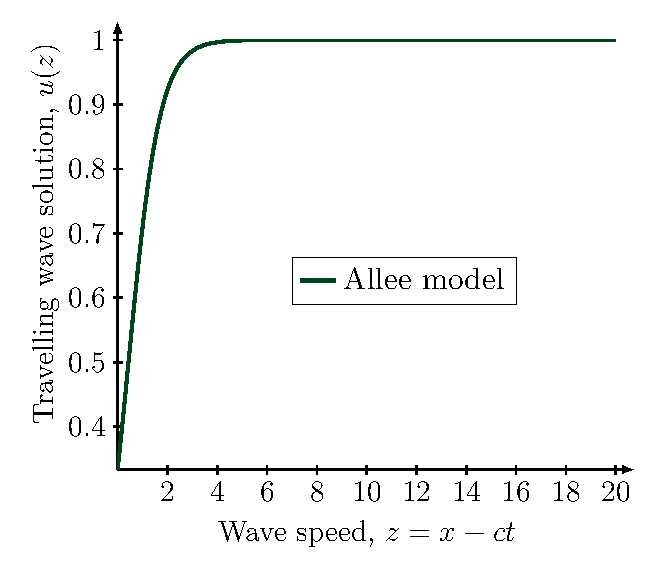
\includegraphics[width=8cm,page=1]{{./individual_figures_travelling_waves}}};
  


\node[inner sep=0pt] (mixed) at (3.75,0)
{\includegraphics[width=8cm,page=2]{{./individual_figures_travelling_waves}}};


\node (b) at (0.35,3.75) { (\textbf{B})};
\node[left=6.67cm of b] (a) {(\textbf{A})};

\end{tikzpicture}

\end{document}
